\documentclass[a4paper]{article}

%% Language and font encodings
\usepackage[english]{babel}
\usepackage[utf8x]{inputenc}
\usepackage[T1]{fontenc}


%% Sets page size and margins
\usepackage[a4paper,top=3cm,bottom=2cm,left=3cm,right=3cm,marginparwidth=1.75cm]{geometry}

%% Useful packages
\usepackage{amsmath}
\usepackage{graphicx}
\usepackage{tikz,pgfplots}
\usepackage[colorinlistoftodos]{todonotes}
\usepackage[colorlinks=true, allcolors=blue]{hyperref}
\usepackage{amsfonts}
\usepackage{bbm}
\usepackage{dsfont}
\usepackage{cancel}
\usepackage{tikz,tkz-base,tkz-fct}
\usepackage{pgfplots}
\newcommand{\prob}{\mathbb{P}}
\newtheorem{definicion}{Definición}
\newtheorem{teorema}{Teorema}
\newtheorem{ejemplo}{Ejemplo}
\DeclareMathOperator*{\argmax}{Arg\,max}
\newtheorem{lem}{Lema}
\newtheorem{prop}{Proposici\'on}
\newtheorem{cor}{Corolario}
\newtheorem{dem}{Demostración}
\numberwithin{equation}{subsection}
\numberwithin{definicion}{subsection}
\newtheorem{obs}{Observación}


%% Aquí se pueden definir nuevas abreviaturas para algunos comandos

\def\sen{{\rm sen\mspace{1.5mu}}}
\def\C{\mathbb C}
\def\R{\mathbb R}
\def\N{\mathbb N}
\def\Q{\mathbb Q}
\def\Z{\mathbb Z}
\def\V{\mathbb V}
\def\E{\mathbb E}
\def\to{\rightarrow}
\newcommand{\pb}{\mathbb{P}}



\newcommand{\ds}{\displaystyle}


%Para hacer normas en tex

\providecommand{\norm}[1]{\lVert#1\rVert}
\providecommand{\normm}[1]{\bigg\lVert#1\bigg\rVert}


%integrales bacanes
\usepackage{ esint }

%Para poner en negrita en modo matemático
\newcommand{\negri}{\boldsymbol}




\title{Simulación Estocástica}
\author{Clase 18}
\date{03 de octubre de 2019}

\begin{document}
\maketitle

\section{Movimiento Browniano, proceso de difusión y aplicaciones}
\subsection{Movimiento Browniano}
La idea general es poder escoger una función (o una asignación) en la variable $t\in \R^{+}$, de manera de poder asegurar la continuidad y mantener la aleatoriedad. En palabras simples, elegir aleatoriamente una función contínua.\\ \newline
Una manera de hacer lo anterior es mediante un \textit{paseo aleatorio}:

\begin{itemize}
    \item Sean $X_1$, $X_2$, $X_3$, $\cdots$ variables aleatorias $i.i.d.$, tales que
    \[\prob(X_i = -1) = \prob(X_i = 1) = \frac{1}{2},\hspace{0.5cm}\forall i \in \N.\hspace{0.3cm}\footnote{En general, cualquier variable aleatoria con $\E(X)=0$ y $Var(X)=1$, puede servir.}\]
    \item $\forall\,n\in \N$,
    \[S_n := \sum_{i=1}^n X_i\,,\hspace{0.5cm}\text{con }S_0 = 0.\]
    \item $\forall\,t\in \R^{+}$, $S_t$ es la interpolación lineal de la colección $(S_n)_{n\in\N}$.
    
    \begin{figure}[h]
    \centering
    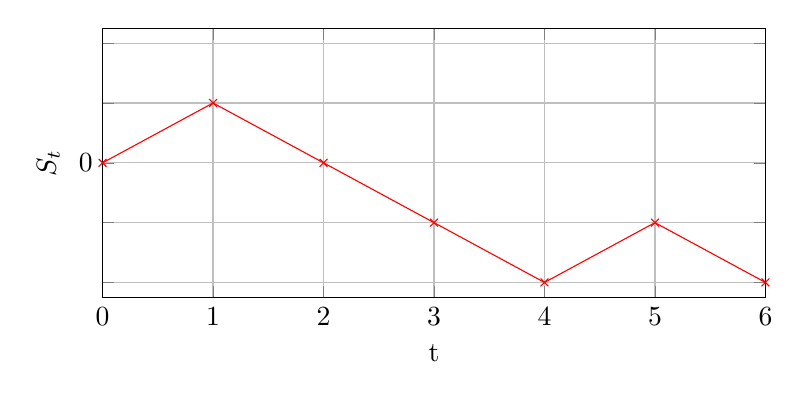
\begin{tikzpicture}
         \begin{axis}
        [width=10cm, height=5cm, xmin=0, xmax=6, ymin=-2.25, ymax=2.25, xmajorgrids=true, ymajorgrids=true, xtick={0,1,2,3,4,5,6}, ytick={-2,-1,0,1,2}, yticklabels={,,0,,},xlabel = t,ylabel = $S_t$]
        \addplot[color=red,mark=x] coordinates {(0,0) (1,1) (2,0) (3,-1) (4,-2) (5,-1) (6,-2)};
        \end{axis}
    \end{tikzpicture}
    \caption{Ejemplo de \textit{Paseo Aleatorio}.}
    \end{figure}
\end{itemize}
 Para valores de $t$ suficientemente grande, y escalando tiempo y espacio adecuadamente, el gráfico de $S_t$ toma la siguiente forma.\\ \newpage
\begin{figure}[h]
    \centering
    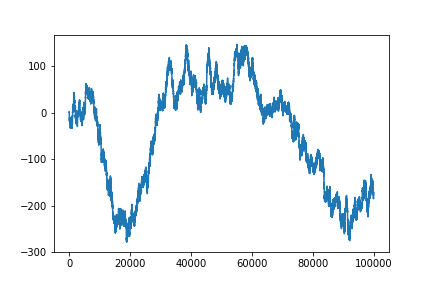
\includegraphics[width=0.6\textwidth]{browniano.png}
\end{figure}

Específicamente, el escalamiento corresponde al siguiente: $\forall\, a>0$, definimos
\[B_t^{(a)}:= \frac{1}{a}S_{ta^2}\]
\newline Estudiaremos la distribución de $B_t^{(a)}$: para $a>0$ fijo y $n\in \N$ (ambos suficientemente grandes), tomar $t=\frac{n}{a^2}$. Luego
\[B_t^{(a)} = \sqrt{\frac{t}{n}}S_n = \sqrt{t}\,\, \frac{1}{\sqrt{n}}\sum_{i=1}^n X_i\]
Ocupando $T.C.L.$, y recordando que $\E(X_i)=0$ y $Var(X_i)=1$, notamos que:
\[\frac{1}{\sqrt{n}}\sum_{i=1}^n X_i \approx Z\,\sim\,\mathcal{N}(0,1), \]
por lo tanto, concluímos que:
\[B_t^{(a)} \approx \sqrt{t}\,\,\mathcal{N}(0,1) = \mathcal{N}(0,t).\]
También es directo ver que, para valores enteros $m>n$, la variable $S_m-S_n$ es independiente de $S_n$ (puesto que la colección $(X_i)_i$ era $i.i.d$), es decir; $(S_n)_{n\in\N}$ posee la propiedad de \textbf{Incrementos Independientes}, lo cual se manifiesta también en $(B_t^{(a)})_{t\geq 0}$. (ver \cite[cap. 2]{Kara})\\ \newline
Lo anterior motiva la siguiente definición.

\begin{definicion}[Movimiento Browniano] Un Movimiento Browniano es un proceso estocástico\footnote{Es decir, una colección de variables aleatorias definidas en algún espacio de probabilidad $(\Omega,\mathcal{F},\prob)$, indexada por la variable $t\geq 0$.}, denotado $(B_t)_{t\geq 0}$, que satisface:
\begin{enumerate}
    \item[i.] $B_0 = 0$, $c.s.$
    \item[ii.] Posee incrementos independientes: $\forall\, t\geq 0$, $(B_{t+s}-B_t)_{s\geq 0}$ es independiente de $(B_s)_{0\leq s\leq t}$.
    \item[iii.] Posee incrementos normales: $\forall\, t,s\geq 0$, $B_{t+s}-B_{t}\,\sim\,\mathcal{N}(0,s)$.
    \item[iv.] Es un proceso contínuo; con probabilidad 1, la función $t\rightarrow\,B_t$ es contínua en $t$.
\end{enumerate}
\end{definicion}

La ley del proceso $(B_t^{(a)})_{t\leq 0}$ converge, cuando $a\rightarrow\,\infty$, a la ley del movimiento browniano $(B_t)_{t\geq 0}$, en un sentido adecuado (Teorema de Donsker, ver \cite[cap.2, Teo.4.2]{Kara}).\\ \newline $(B_t)_{t\geq 0}$ también es llamado \textbf{Proceso de Weiner}. El nombre "browniano" fue puesto en honor al botánico escocés, Robert Brown, quién observó el movimiento errático de partículas de polen en el agua en 1827. Porsteriormente, en 1905, el físico Albert Einstein explicaría este movimiento como resultado  de muchas pequeñas colisiones de polen con las moléculas de agua circundantes.\\ \newline
Pero, ¿realmente existe un proceso tal que cumpla $i$, $ii$, $iii$, y $iv$, de la difinición anterior?
\begin{teorema}
El Movimiento Browniano existe.
\end{teorema}
\textbf{Demostración: }ver \cite[cap. 2]{Kara}.\\ \newline

\begin{prop}Sea $(B_t)_{t\geq 0}$ Movimiento Browniano ($M.B.$), $\forall\, 0=t_0<t_1<t_2<\cdots<t_n$, la colección
\[\left(\frac{B_{t_i}-B_{t_{i-1}}}{\sqrt{t_i-t_{i-1}}}\right)_{i=1,\cdots,n}\]
son $i.i.d.$ $\mathcal{N}(0,1)$.
\end{prop}
\textbf{Demostración: }Directo de la definición de $M.B$.\\\rule{0.7em}{0.7em}\\ \newline
Esto da lugar  a un método sencillo para generar un $M.B.$ discretizado: para un horizonte $T>0$, y $n\in\N$, sea $\Delta t = T/n$, y $t_i = i\Delta t$. Dado $Z_1,\cdots, Z_n$,  $i.i.d.$ $\mathcal{N}(0,1)$, entonces el proceso $(Y_t)_{t\in [0,T]}$, definido como 
\[Y_{t_i}:= \sqrt{\Delta t}\,\sum_{j=1}^i Z_i\]
interpolando linealmente entre los $t_i$'s para los valores en $[0,T]\backslash\{t_0,\cdots,t_n\}$, es una aproximación de $(B_t)_{t\in[0,T]}$ (de hecho, tiene la misma ley en la malla $0=t_0<t_1<\cdots<t_n=T$).

\begin{prop} Sea $(B_t)_{t\geq 0}$ un $M.B.$:
\begin{enumerate}
    \item[a.] $\forall\,t_0>0$, el proceso $X_t := B_{t+t_0}-B_{t_0}$ es un $M.B.$. (Invarianza bajo shift)
    \item[b.] $\forall\,c>0$, el proceso $X_t := \frac{1}{\sqrt{c}}\,B_{ct}$ es un $M.B.$ (Invarianza bajo escalamiento)
    \item[c.] El proceso $X_t := B_1 - B_{1-t}$ es un $M.B.$ en $[0,1]$. (Propiedad de tiempo reverso)
    \item[d.]  El proceso $X_t:=tB_{1/t}$ es un $M.B.$ (con $X_0 =0$). (Inversión del tiempo)
    \item[e.] el proceso $X_t:=-B_t$ es un $M.B.$ (Simetría)
\end{enumerate}
\end{prop}
\textbf{Demostración: }ver \cite[cap. 2]{Kara}.\\ \newline
A pesar de ser contínuas, las trayectorias de un movimiento browniano son bastante irregulares. La \textit{trayectoria} de un $M.B.$ es la función (aleatoria)
\[t\rightarrow\,B_t\]
\begin{teorema}
\[\prob\left(\exits\,t\geq 0\,:\,B_t\,\text{es derivable en }t\right) = 0\]
\end{teorema}
\end{document}